\documentclass[11pt,french,french]{article}
\usepackage{lmodern}
\usepackage{amssymb,amsmath}
\usepackage{ifxetex,ifluatex}
\usepackage{fixltx2e} % provides \textsubscript
\ifnum 0\ifxetex 1\fi\ifluatex 1\fi=0 % if pdftex
  \usepackage[T1]{fontenc}
  \usepackage[utf8]{inputenc}
\else % if luatex or xelatex
  \ifxetex
    \usepackage{mathspec}
    \usepackage{xltxtra,xunicode}
  \else
    \usepackage{fontspec}
  \fi
  \defaultfontfeatures{Mapping=tex-text,Scale=MatchLowercase}
  \newcommand{\euro}{€}
\fi
% use upquote if available, for straight quotes in verbatim environments
\IfFileExists{upquote.sty}{\usepackage{upquote}}{}
% use microtype if available
\IfFileExists{microtype.sty}{%
\usepackage{microtype}
\UseMicrotypeSet[protrusion]{basicmath} % disable protrusion for tt fonts
}{}
\usepackage[margin=0.95in]{geometry}
\ifxetex
  \usepackage{polyglossia}
  \setmainlanguage{}
\else
  \usepackage[shorthands=off,french]{babel}
\fi
\usepackage{graphicx}
\makeatletter
\def\maxwidth{\ifdim\Gin@nat@width>\linewidth\linewidth\else\Gin@nat@width\fi}
\def\maxheight{\ifdim\Gin@nat@height>\textheight\textheight\else\Gin@nat@height\fi}
\makeatother
% Scale images if necessary, so that they will not overflow the page
% margins by default, and it is still possible to overwrite the defaults
% using explicit options in \includegraphics[width, height, ...]{}
\setkeys{Gin}{width=\maxwidth,height=\maxheight,keepaspectratio}
\ifxetex
  \usepackage[setpagesize=false, % page size defined by xetex
              unicode=false, % unicode breaks when used with xetex
              xetex]{hyperref}
\else
  \usepackage[unicode=true]{hyperref}
\fi
\hypersetup{breaklinks=true,
            bookmarks=true,
            pdfauthor={},
            pdftitle={},
            colorlinks=true,
            citecolor=blue,
            urlcolor=blue,
            linkcolor=magenta,
            pdfborder={0 0 0}}
\urlstyle{same}  % don't use monospace font for urls
\setlength{\parindent}{0pt}
\setlength{\parskip}{6pt plus 2pt minus 1pt}
\setlength{\emergencystretch}{3em}  % prevent overfull lines
\setcounter{secnumdepth}{5}

%%% Use protect on footnotes to avoid problems with footnotes in titles
\let\rmarkdownfootnote\footnote%
\def\footnote{\protect\rmarkdownfootnote}


  \title{Sentimental analysis}
    \author{Romain Lesauvage}
    \date{}
  
\usepackage{caption}
\usepackage{graphicx}
\usepackage{natbib}

\begin{document}

\maketitle


Nous souhaitons désormais utiliser les \emph{word-embeddings} obtenus
afin d'implémenter un modèle de \emph{sentimental analysis}. Nous
disposons pour cela d'une nouvelle base de données, constituée de tweets
anglais traduits en français et annotés, avec 0 pour les tweets
\og négatifs \fg et 4 pour les tweets \og positifs \fg. Elle est
découpée en deux fichiers : un d'entraînement avec plus d'1,5 millions
de tweets et une de test avec 4000 de tweets. Il a été retenu de garder
50000 tweets du fichier d'entraînement pour entraîner nos modèles, en
faisant bien attention à garder un fichier équilibré, c'est-à-dire avec
autant de tweets positifs que négatifs. Nous avons également transformé
la valeur 0 en -1 et la valeur 4 en 1 pour les sentiments.

\section{Description du modèle}\label{description-du-moduxe8le}

Afin d'exploiter nos vecteurs, l'idée est de réaliser une régression
logistique sur la base d'entraînement, en considérant comme prédicteurs
chacune des dimensions des vecteurs. Pour réaliser cela, il faut
toutefois pouvoir attribuer à chaque tweet un vecteur, réaliser une
forme de \emph{sentence embedding}. Dans une première approche, nous
avons décidé d'attribuer à chaque tweet la moyenne des vecteurs de
l'ensemble des mots. Nous pouvons ensuite réaliser la régression sur ce
vecteur.

Si on note \(Y_i\) le sentiment du tweet (noté \emph{polarity} dans la
base), et \(X_{i,1}, \dots, X_{i,n}\) chacune des coordonnées du vecteur
de la phrase, alors nous allons chercher à estimer :

\begin{equation}
\log\left(\frac{\mathbb{P}(Y_i = 1)}{1 - \mathbb{P}(Y_i = 1)}\right) = \beta_0 + \sum\limits_{i = 0}^n \beta_i X_{i,j}
\end{equation}

Cependant, une fois ce modèle estimé, il faudra pouvoir estimer son
efficacité. Pour cela, on décide donc de s'intéresser à deux modèles
plus simples, ne faisant pas appel aux \emph{word-embeddings}, qui nous
serviront de référence.

\section{Modèles de référence}\label{moduxe8les-de-ruxe9fuxe9rence}

\subsection{Modèle aléatoire}\label{moduxe8le-aluxe9atoire}

Le premier modèle de référence auquel on peut penser est le modèle
aléatoire, c'est-à-dire celui qui attribue à chaque tweet le sentiment 1
ou -1 avec la probabilité \(\frac{1}{2}\). On obtient avec ce modèle une
précision de \textbf{50,15 \%}.

\begin{figure}
\centering
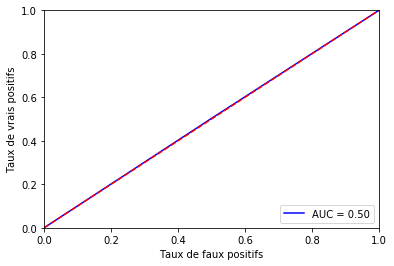
\includegraphics{img/roc_random.png}
\caption{Courbe ROC pour modèle aléatoire}
\end{figure}

\subsection{Modèle avec sentiment moyen des
mots}\label{moduxe8le-avec-sentiment-moyen-des-mots}

Le modèle aléatoire n'est évidemment pas satisfaisant. Il peut cependant
être amélioré car il ne prend pas en compte les informations disponibles
dans les données, à savoir les tweets annotés. Nous pouvons donc penser
à un autre modèle qui utilisera cette information. Pour cela, on
raisonne en trois temps :

\begin{itemize}
\item On commence par calculer un sentiment moyen par mot, en prenant la moyenne des sentiments des tweets dans lesquels le mot intervient ;
\item On calcule ensuite pour chaque tweet le sentiment moyen des mots de la phrase ($s$);
\item On définit ensuite une réglère de décision du type $\mathbb{I}(s \geq \alpha)$ avec un paramètre $\alpha$ à optimiser.
\end{itemize}

On implémente donc cela et on cherche à optimiser la valeur de
\(\alpha\). En représentant la précision sur les bases de \emph{train}
et \emph{test} pour toutes les valeurs de \(\alpha\) entre -1 et 1 (avec
un pas de 0,1), on trouve que \(\alpha_{opti} = -0.05\).

\begin{figure}
\centering
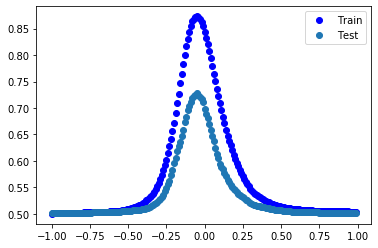
\includegraphics{img/choix_alpha.png}
\caption{Choix du meilleur alpha}
\end{figure}

Avec cette valeur de \(\alpha\), on obtient alors une précision de
\textbf{87,33 \%} sur le \emph{train} et \textbf{72,90 \%} sur le
\emph{test}.

\begin{figure}
\centering
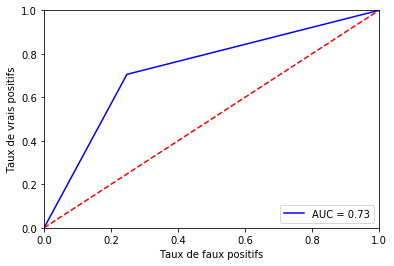
\includegraphics{img/roc_sentiments.png}
\caption{Courbe ROC pour modèle sentiment moyen des mots}
\end{figure}

A ce stade, nous avons donc notre seuil pour évaluer notre modèle. En
effet, nous aimerions idéalement que notre modèle basé sur les
\emph{word-embeddings} fasse mieux que le modèle avec sentiment moyen
des mots, donc \textbf{nous aimerions une précision supérieure à 72,9 \%
sur le test}.

\subsection{\texorpdfstring{Modèle basé sur
\textbf{word-embeddings}}{Modèle basé sur word-embeddings}}\label{moduxe8le-basuxe9-sur-word-embeddings}

On utilise maintenant les vecteurs obtenus grâce au modèle
\emph{Word2Vec}. Comme indiqué, on effectue la régression logistique du
sentiment sur le vecteur moyen de la phrase. Puisque nous avons des
résultats pour différentes dimensions (50, 100 et 300), nous allons
tester les 3. Par ailleurs, nous avons à disposition 6 seeds par
dimension, nous utiliserons donc les vecteurs moyens de ces 6 seeds.

On obtient alors les résultats suivants :

\begin{center}
\begin{tabular}{| c || c | c |}
\hline
Dimension & Précision - Train (\%)) & Précision - Test (\%)) \\ \hline
50 & 67,98 & 67,05 \\ \hline
100 & 69,19 & 68,71 \\ \hline
300 & 71,64 & 70,39 \\ \hline
\end{tabular}
\end{center}

\begin{figure}
\centering
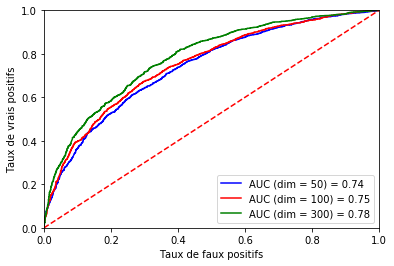
\includegraphics{img/roc_word.png}
\caption{Courbe ROC pour modèle sur \emph{word-embedding}}
\end{figure}

On remarque donc, comme attendu, que le résultat est moins bien sur la
base test que celle d'entraînement, mais de très peu. Plus la dimension
augmente, meilleurs sont les résultats. Toutefois, même en dimension
300, on se rapproche des résultats du modèle sur le sentiment moyen des
mots mais reste légèrement moins bien.

Afin d'améliorer les résultats, nous tentons d'enlever les \emph{stop
words} qui, a priori, n'apportent pas d'informations sur le sentiment
d'un tweet. On obtient les résultats suivants :

\begin{center}
\begin{tabular}{| c || c | c |}
\hline
Dimension & Précision - Train (\%)) & Précision - Test (\%)) \\ \hline
50 & 66,42 & 65,85 \\ \hline
100 & 67,64 & 66,88 \\ \hline
300 & 70,08 & 69,54 \\ \hline
\end{tabular}
\end{center}

\begin{figure}
\centering
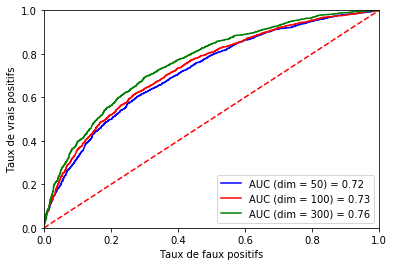
\includegraphics{img/roc_word_st.png}
\caption{Courbe ROC pour modèle sur \emph{word-embedding} en enlevant
les \emph{stop words}}
\end{figure}

Les résultats ne sont pas meilleurs, ils sont même légèrement moins bon,
donc cette approche n'est pas validée. Nous tentons alors de voir
désormais si la normalisation des vecteurs peut avoir un impact. Nous
réalisons les mêmes expériences :

\begin{center}
\begin{tabular}{| c || c | c |}
\hline
Dimension & Précision - Train (\%)) & Précision - Test (\%)) \\ \hline
50 & 68,32 & 67,23 \\ \hline
100 & 69,15 & 69,09 \\ \hline
300 & 71,49 & 70,49 \\ \hline
\end{tabular}
\end{center}

\begin{figure}
\centering
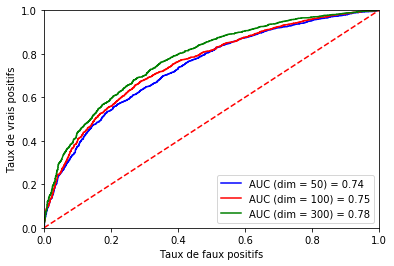
\includegraphics{img/roc_word_norm.png}
\caption{Courbe ROC pour modèle sur \emph{word-embedding} en normalisant
les vecteurs}
\end{figure}

Encore une fois, on obtient des résultats similaires, bien que très
légèrement meilleurs au modèle non normalisé. \newline Afin d'améliorer
les résultats, une dernière idée pourrait être d'utiliser dans la
régression logistique les sentiments moyens calculés pour chaque mot, en
pondérant chaque mot dans une phrase par son sentiment dans le calcul de
l'\emph{embedding} moyen de la phrase. On obtient alors les résultats
qui suivent :

\begin{center}
\begin{tabular}{| c || c | c |}
\hline
Dimension & Précision - Train (\%)) & Précision - Test (\%)) \\ \hline
50 & 78,83 & 68,96 \\ \hline
100 & 79,72 & 69,01 \\ \hline
300 & 81,42 & 71,02 \\ \hline
\end{tabular}
\end{center}

\begin{figure}
\centering
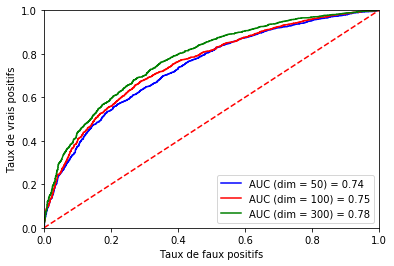
\includegraphics{img/roc_word_norm.png}
\caption{Courbe ROC pour modèle sur \emph{word-embedding} en pondérant
par sentiment des mots}
\end{figure}

Les résultats s'améliorent un peu, mais on est encore légèrement
en-dessous du modèle de référence.

\section{Conclusion}\label{conclusion}

En conclusion, quelque soit le modèle logistique utilisé, les résultats
sont très proches et légèrement moins bien que le modèle de référence.
Le meilleur résultat est toutefois obtenu pour le modèle pondéré par les
sentiments des mots et pour une dimension de 300. On peut donc décider
d'utiliser cette dimension pour la suite. Même si notre modèle ne semble
pas améliorer les performances par rapport au modèle sans
\emph{word-embedding}, il faudrait pouvoir le tester sur une autre base
annotée pour mesurer cet écart, car dans le corpus actuel environ un mot
sur deux n'a pas été entraîné par \emph{Word2Vec}. Afin d'améliorer
également les performances, il faut améliorer le préprocessing de la
base.

\end{document}